\documentclass[tikz, border=5mm]{standalone}
\usetikzlibrary{calc}

% Definición explícita de colores
\definecolor{myorange}{RGB}{255, 127, 0}

\begin{document}
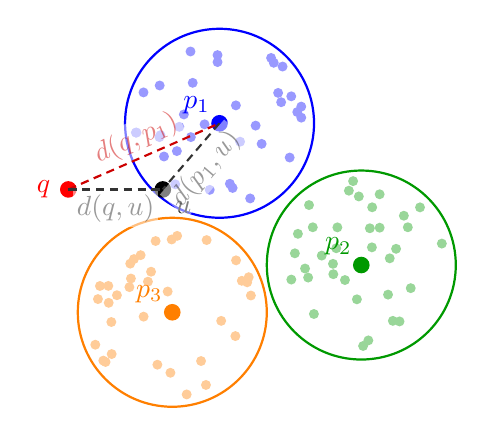
\begin{tikzpicture}[scale=1.2]

    % Fijar semilla para reproducibilidad
    \pgfmathsetseed{12345}

    % --- Parámetros globales ---
    \def\r{1.0} % Radio de los círculos de cobertura
    \def\npoints{35} % Puntos por clúster

    % --- Definición de los 3 pivotes (índice, x, y, color) ---
    % Distribución en forma de triángulo
    \foreach \i/\px/\py/\c in {
        1/3.0/4.5/blue,
        2/4.5/3/green!60!black,
        3/2.5/2.5/myorange}{
        % 1. Definir la coordenada del pivote
        \coordinate (p\i) at (\px, \py);
        
        % 2. Dibujar el círculo de cobertura (apretado a la nube)
        \draw[\c, thick] (p\i) circle (\r);
        
        % 3. Generar la nube de puntos mediante coordenadas polares
        \foreach \j in {1,...,\npoints} {
            % El radio máximo es r * 0.9 para asegurar que los puntos no toquen el borde
            \pgfmathsetmacro{\rad}{\r * 0.9 * sqrt(rnd)}
            \pgfmathsetmacro{\ang}{360*rnd}
            \fill[\c!40] ($(p\i) + (\ang:\rad)$) circle (1.5pt);
        }
        
        % 4. Dibujar el pivote y su etiqueta
        \fill[\c] (p\i) circle (2.5pt) node[above left, font=\bfseries] {$p_\i$};
    }

    % --- Elementos de consulta y triangulación ---

    % Punto de consulta 'q' acercado al clúster p1
    \coordinate (q) at (1.4, 3.8);
    \fill[red] (q) circle (2.5pt) node[left=3pt, font=\bfseries] {$q$};

    % Punto 'u' ubicado dentro de la cobertura de p1
    \coordinate (u) at (2.4, 3.8);
    \fill[black] (u) circle (2.5pt) node[below right=1pt, font=\bfseries] {$u$};

    % Trazar la triangulación entre q, u y p1
    % q -> p1 (Línea superior del triángulo)
    \draw[thick, densely dashed, red!80!black] (q) -- (p1) 
        node[midway, fill=white, inner sep=1.5pt, sloped, above, opacity=0.5] {$d(q, p_1)$};
        
    % q -> u (Línea horizontal inferior)
    \draw[thick, densely dashed, black!80] (q) -- (u) 
        node[midway, fill=white, inner sep=1.5pt, sloped, below, opacity=0.5] {$d(q, u)$};
        
    % p1 -> u (Línea inclinada derecha)
    \draw[thick, densely dashed, black!80] (p1) -- (u) 
        node[midway, fill=white, inner sep=1.5pt, sloped, below, opacity=0.5] {$d(p_1, u)$};

\end{tikzpicture}
\end{document}
